\section{梯度下降}
\label{sec:fom-gradient-descent}

只知道当前点的函数值和梯度，下一步应该朝哪里走、走多远？本节回答这个问题，并分三种情形说明这样走能得到什么：一般非凸、凸、强凸。三种情形的结论强弱不同，度量误差的尺子也不同。

\paragraph{主要思想}
先看方向。在$\bm{x}$附近，目标由一阶Taylor展开近似：
\[
 f(\bm{x}+\bm{d})\approx f(\bm{x})+\nabla f(\bm{x})^\top\bm{d}.
\]
在固定长度的$\bm{d}$中，要让$\nabla f(\bm{x})^\top\bm{d}$最小。由Cauchy--Schwarz不等式，
\[
 \nabla f(\bm{x})^\top\bm{d}\geq-\lVert\nabla f(\bm{x})\rVert_2\lVert\bm{d}\rVert_2,
\]
等号当且仅当$\bm{d}$与$-\nabla f(\bm{x})$同向时成立。所以局部最陡的下降方向是负梯度方向。

线性模型只给方向，不给距离：沿负梯度走得越远，线性模型的值越低，没有尽头。真实的地面会弯曲，线性预测走远了就不可信。需要一个量来说明“能信多远”。

这个量就是第~\ref{chap:smooth-foundations}章的光滑常数$L$，它要求梯度满足Lipschitz条件：
\[
 \lVert\nabla f(\bm{x})-\nabla f(\bm{y})\rVert_2\leq L\lVert\bm{x}-\bm{y}\rVert_2.
\]

在这个条件下，下降引理给出处处成立的二次上界：
\begin{equation}
 f(\bm{y})\leq f(\bm{x})+\nabla f(\bm{x})^\top(\bm{y}-\bm{x})+\frac{L}{2}\lVert\bm{y}-\bm{x}\rVert_2^2.
 \label{eq:fom-descent-lemma}
\end{equation}
二阶可微时，$\nabla^2f\preceq L\bm{I}$且$\nabla^2f\succeq-L\bm{I}$就保证了这一点。可以把右端想成扣在地面上的一只碗：它在$\bm{x}$处贴住地面，其余地方都不低于地面。

既然地面不高于这只碗，就走到碗底。对$\bm{y}$求右端的最小点，令导数为零，得到$\bm{y}=\bm{x}-\nabla f(\bm{x})/L$。图~\ref{fig:fom-upper-bound}画的是一元的情形：绿色的碗底对应的横坐标就是新点，碗底的高度保证了至少下降多少。

\begin{BookInlineFigure}
  \centering
  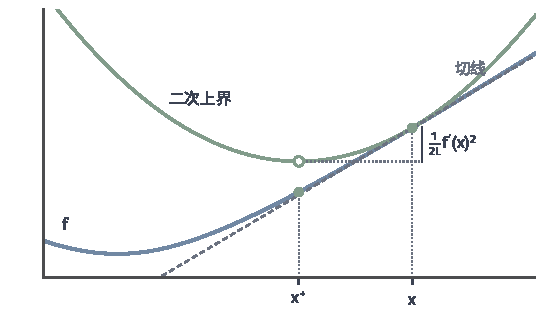
\includegraphics[width=92mm]{figures/05-optimization/02-smooth-optimization/matplotlib/fom-upper-bound/figure.pdf}
  \caption{二次上界决定一步走多远。蓝色曲线是$f(x)=\sqrt{1+x^2}$，它的二阶导数不超过$1$，取$L=1$。虚线是$x=2.4$处的切线，绿色抛物线是式~\eqref{eq:fom-descent-lemma}的上界。空心点是上界的最低点，其横坐标$x^{+}$就是新点，实心点是真实的函数值，它不高于空心点。竖线段是保证的下降量。}
  \label{fig:fom-upper-bound}
\end{BookInlineFigure}

把步长放宽为任意的$\alpha>0$，就得到\term{梯度下降法}（gradient descent method）：
\begin{equation}
 \bm{x}^{(t+1)}=\bm{x}^{(t)}-\alpha^{(t)}\bm{g}^{(t)},\qquad \bm{g}^{(t)}=\nabla f(\bm{x}^{(t)}).
 \label{eq:fom-gd}
\end{equation}
把$\bm{y}=\bm{x}^{(t+1)}$代入式~\eqref{eq:fom-descent-lemma}，一阶项是$-\alpha\lVert\bm{g}^{(t)}\rVert_2^2$，二次项是$\tfrac{L}{2}\alpha^2\lVert\bm{g}^{(t)}\rVert_2^2$，合起来得到单步下降估计：
\begin{equation}
 f(\bm{x}^{(t+1)})\leq f(\bm{x}^{(t)})-\alpha\Bigl(1-\frac{L\alpha}{2}\Bigr)\lVert\bm{g}^{(t)}\rVert_2^2.
 \label{eq:fom-gd-decrease}
\end{equation}
只要$0<\alpha<2/L$，括号就是正的，函数值严格下降。关于$\alpha$求最大的下降量，得到$\alpha=1/L$，此时每步至少下降$\lVert\bm{g}^{(t)}\rVert_2^2/(2L)$。

步长的来源有三种，都沿用第~\ref{chap:smooth-foundations}章的规则。已知$L$时取固定步长；不知道$L$时用回溯，从一个试探值开始不断缩短，直到满足Armijo条件
\begin{equation}
 f(\bm{x}+\alpha\bm{d})\leq f(\bm{x})+c_1\alpha\nabla f(\bm{x})^\top\bm{d},\qquad 0<c_1<1;
 \label{eq:fom-armijo}
\end{equation}
二次目标上还可以精确求沿线最小点。负梯度方向的精确步长是
\[
 \alpha=\frac{\bm{g}^\top\bm{g}}{\bm{g}^\top\bm{H}\bm{g}},
\]
这时的方法称为最速下降法（steepest descent）。

\needspace{6\baselineskip}
\paragraph{变量}
\begin{itemize}
 \item $\bm{x}^{(t)}\in\mathbb{R}^n$：当前点，在原处更新。
 \item $\bm{g}^{(t)}\in\mathbb{R}^n$：当前点的梯度，每轮读取一次。
 \item $\alpha>0$：步长，这里固定；用线搜索时每轮重新确定。
 \item $\varepsilon>0$，$T$：梯度大小的容差与最大步数。
\end{itemize}

\paragraph{初始化}
选定起点$\bm{x}^{(0)}$、步长、容差，令$t=0$。例中用式~\eqref{eq:fom-example}的起点，并取$\alpha=1/5$（下文说明这个值从哪里来），容差$\varepsilon=10^{-3}$。初始值是
\[
 \bm{x}^{(0)}=(9,1),\qquad f(\bm{x}^{(0)})=45.
\]

\needspace{6\baselineskip}
\paragraph{每轮更新}
在第$t$轮：
\begin{enumerate}
 \item \textbf{读取梯度。}计算$\bm{g}^{(t)}=\nabla f(\bm{x}^{(t)})$。例中$\nabla f(\bm{x})=(x_1,9x_2)$，第一轮
 \[
  \bm{g}^{(0)}=(9,9).
 \]
 \item \textbf{检查停止。}若$\lVert\bm{g}^{(t)}\rVert_2\leq\varepsilon$或$t=T$，输出$\bm{x}^{(t)}$并结束。例中第一轮$\lVert\bm{g}^{(0)}\rVert_2=9\sqrt2\approx12.73$，继续。
 \item \textbf{更新。}按式~\eqref{eq:fom-gd}计算新点，令$t\leftarrow t+1$。例中第一轮
 \[
  \bm{x}^{(1)}=(9,1)-\tfrac15(9,9)=(7.2,-0.8),\qquad f(\bm{x}^{(1)})=28.8.
 \]

 例中第二轮$\bm{g}^{(1)}=(7.2,-7.2)$，于是
 \[
  \bm{x}^{(2)}=(7.2,-0.8)-\tfrac15(7.2,-7.2)=(5.76,0.64),
 \]
 目标值$f(\bm{x}^{(2)})=18.432$。

 例中第三轮$\bm{g}^{(2)}=(5.76,5.76)$，于是
 \[
  \bm{x}^{(3)}=(5.76,0.64)-\tfrac15(5.76,5.76)=(4.608,-0.512),
 \]
 目标值$f(\bm{x}^{(3)})=11.79648$。
\end{enumerate}

规律已经显出来了：两个坐标分别乘以$1-\alpha\lambda$，第一个因子是$1-\tfrac15=0.8$，第二个因子是$1-\tfrac95=-0.8$。因此
\[
 \bm{x}^{(t)}=0.8^t\bigl(9,(-1)^t\bigr),\qquad f(\bm{x}^{(t)})=45\cdot0.64^t.
\]

梯度大小是$\lVert\bm{g}^{(t)}\rVert_2=0.8^t\cdot9\sqrt2$，它不超过$10^{-3}$要求$t\geq43$。最终得到
\[
 \bm{x}^{(43)}\approx(6.13\times10^{-4},\,-6.81\times10^{-5}).
\]
这个起点是特意选的：沿$\bm{d}=-\bm{g}$的精确步长恰好处处等于$1/5$，所以这串点也是最速下降的结果。

\paragraph{步长与收缩因子}
为什么取$1/5$，而不是上界推出的$1/L=1/9$？这要看二次目标上一步到底做了什么。设
\[
 f(\bm{x})=\frac12(\bm{x}-\bm{x}^\star)^\top\bm{H}(\bm{x}-\bm{x}^\star)+f^\star,
\]
其中$\bm{H}$对称正定，特征值都落在$[\mu,L]$内。记$\bm{e}^{(t)}=\bm{x}^{(t)}-\bm{x}^\star$，由$\bm{g}^{(t)}=\bm{H}\bm{e}^{(t)}$得
\[
 \bm{e}^{(t+1)}=(\bm{I}-\alpha\bm{H})\bm{e}^{(t)}.
\]

用$\bm{H}$的标准正交特征向量作坐标，矩阵变成对角形，每个特征方向各自演化。特征值为$\lambda$的分量每步乘以同一个数：
\begin{equation}
 e_\lambda^{(t+1)}=(1-\alpha\lambda)\,e_\lambda^{(t)}.
 \label{eq:fom-gd-factor}
\end{equation}
特征分解的做法可参考\BookChapterRef{chap:eigen-spectral-decomposition}{卷二第6章“谱分解”}。

步长是所有方向共用的一个数，而不同方向希望的步长不同：$\lambda$方向最想要$\alpha=1/\lambda$，一步到位。图~\ref{fig:fom-step-factor}把例中两个方向的因子画在一起。陡峭方向的折线下降得快，在$\alpha=1/9$处触底，随后反弹；平坦方向的线缓慢下降。整体的进度取决于两条线中较高的那条。

\begin{BookInlineFigure}
  \centering
  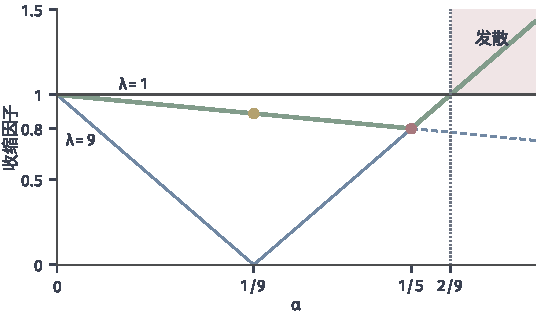
\includegraphics[width=92mm]{figures/05-optimization/02-smooth-optimization/matplotlib/fom-step-factor/figure.pdf}
  \caption{贯穿例上两个特征方向的收缩因子$\lvert1-\alpha\lambda\rvert$。蓝色实线对应陡峭方向$\lambda=9$，蓝色虚线对应平坦方向$\lambda=1$，绿色粗线是两者的较大值。黄点是$\alpha=1/L=1/9$，红点是使较大值最小的$\alpha=2/(L+\mu)=1/5$，此时因子等于$0.8$。红底区域$\alpha>2/9$中因子超过$1$，迭代发散。}
  \label{fig:fom-step-factor}
\end{BookInlineFigure}

要让最慢的方向尽量快，就让两条线相交。这件事可以写成一条定理。

\begin{theorem}[二次目标上的最佳固定步长]
\label{thm:fom-gd-quadratic}
设$\bm{H}$对称正定，特征值落在$[\mu,L]$内，且$\mu$和$L$都是特征值。固定步长的梯度下降收敛到$\bm{x}^\star$（对任意起点）当且仅当$0<\alpha<2/L$。取$\alpha=2/(L+\mu)$时，最大收缩因子最小，并且
\begin{equation}
 \lVert\bm{x}^{(t)}-\bm{x}^\star\rVert_2\leq\Bigl(\frac{\kappa-1}{\kappa+1}\Bigr)^t\lVert\bm{x}^{(0)}-\bm{x}^\star\rVert_2.
 \label{eq:fom-gd-quadratic-rate}
\end{equation}
\end{theorem}

\begin{proof}
由式~\eqref{eq:fom-gd-factor}，第$t$步的$\lambda$分量等于$(1-\alpha\lambda)^t$乘以初值。任意起点都收敛，当且仅当对每个特征值都有$\lvert1-\alpha\lambda\rvert<1$，即$0<\alpha\lambda<2$。这在$\lambda=L$时最严格，所以条件是$0<\alpha<2/L$。

函数$\lvert1-\alpha\lambda\rvert$关于$\lambda$是凸的，在$[\mu,L]$上的最大值在端点取得，所以最大因子是
\[
 \rho(\alpha)=\max\{\lvert1-\alpha\mu\rvert,\lvert1-\alpha L\rvert\}.
\]

随着$\alpha$增大，$1-\alpha\mu$减小，$\alpha L-1$增大。两者相等时最大值最小，这时$1-\alpha\mu=\alpha L-1$，解得
\[
 \alpha=\frac{2}{L+\mu},\qquad \rho=1-\frac{2\mu}{L+\mu}=\frac{\kappa-1}{\kappa+1}.
\]

最后，标准正交变换保持欧氏长度，各分量的平方和至多缩小$\rho^2$倍，即得结论。
\end{proof}

例中$\kappa=9$，$\rho=8/10=0.8$，正是上面算出的因子。起点$(9,1)$使两个方向同时达到这一因子，所以界~\eqref{eq:fom-gd-quadratic-rate}在这个例子上取等号。

图~\ref{fig:fom-gd-paths}把步长的影响画在等高线上。$\alpha=1/9$时第一步就消掉了$x_2$，随后沿谷底以因子$8/9$慢慢前进，路径光滑但慢；$\alpha=1/5$时路径左右折返，前进因子却是$0.8$；$\alpha=0.23$超过了$2/9$，$x_2$每步乘以$-1.07$，折返幅度越来越大。

\begin{BookInlineFigure}
  \centering
  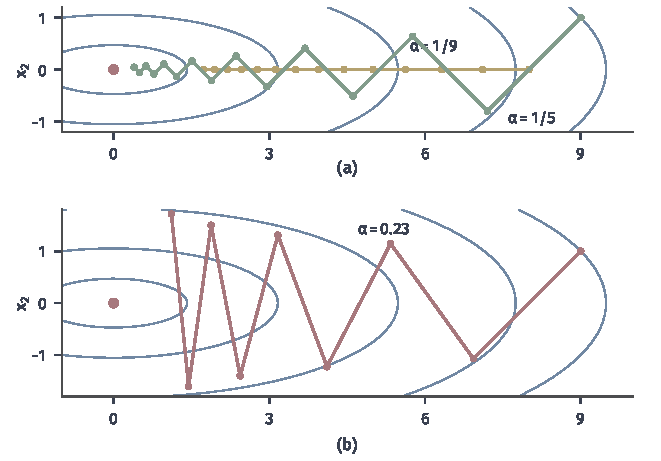
\includegraphics[width=112mm]{figures/05-optimization/02-smooth-optimization/matplotlib/fom-gd-paths/figure.pdf}
  \caption{贯穿例上不同固定步长的路径，蓝色椭圆是等高线，红点是最优解。(a)黄色路径$\alpha=1/9$，绿色路径$\alpha=1/5$，各走$14$步。(b)红色路径$\alpha=0.23>2/L$，走$8$步，$x_1$在收缩，$x_2$的振幅却在放大。}
  \label{fig:fom-gd-paths}
\end{BookInlineFigure}

于是$\alpha=1/L$与$\alpha=2/(L+\mu)$回答的是两个不同的问题。前者由上界推出，只用$L$，保证函数值每步下降，下面的定理都以它为基础；后者要同时知道$\mu$和$L$，它在二次目标上收缩最快，函数值也下降，但路径来回摆动。

\paragraph{一般非凸情形：梯度残差}
下面离开二次目标。先看最弱的假设：$f$可以非凸，只要求梯度Lipschitz，并且有下界。这时目标差和解距离都无从谈起，因为可能有许多局部的谷底，能评价的只有梯度的大小。

\begin{theorem}[非凸情形的梯度下降]
\label{thm:fom-gd-nonconvex}
设$f$的梯度$L$-Lipschitz连续，$f_{\inf}=\inf f>-\infty$。取固定步长$\alpha=1/L$，则对任意$T\geq1$，
\begin{equation}
 \min_{0\leq t<T}\lVert\bm{g}^{(t)}\rVert_2^2\leq\frac{2L\bigl(f(\bm{x}^{(0)})-f_{\inf}\bigr)}{T},
 \label{eq:fom-gd-nonconvex}
\end{equation}
并且$\lVert\bm{g}^{(t)}\rVert_2\to0$，$\{\bm{x}^{(t)}\}$的每个极限点都是驻点。
\end{theorem}

\begin{proof}
由式~\eqref{eq:fom-gd-decrease}，取$\alpha=1/L$时每步满足
\[
 \frac{1}{2L}\lVert\bm{g}^{(t)}\rVert_2^2\leq f(\bm{x}^{(t)})-f(\bm{x}^{(t+1)}).
\]

对$t=0,\ldots,T-1$求和，右端裂项，再用$f(\bm{x}^{(T)})\geq f_{\inf}$，得到
\[
 \frac{1}{2L}\sum_{t=0}^{T-1}\lVert\bm{g}^{(t)}\rVert_2^2\leq f(\bm{x}^{(0)})-f_{\inf}.
\]

$T$项的最小值不超过平均值，这就是式~\eqref{eq:fom-gd-nonconvex}。令$T\to\infty$，上式说明级数$\sum\lVert\bm{g}^{(t)}\rVert_2^2$收敛，所以通项趋于零。$\nabla f$连续，极限点处的梯度等于梯度序列的极限，也就是零。
\end{proof}

定理说的是“某一步的梯度够小”，并没有说最后一步最小，所以输出时要记住梯度最小的那个迭代点。换成任意$\alpha\in(0,2/L)$，只需把$1/(2L)$换成$\alpha(1-L\alpha/2)$。

用回溯时结论同样成立，只差常数。由式~\eqref{eq:fom-gd-decrease}，凡是$\alpha\leq2(1-c_1)/L$的步长都满足Armijo条件。所以若初始试探值为$\alpha_0$、每次缩短到$\rho$倍，接受的步长不低于$\min\{\alpha_0,2\rho(1-c_1)/L\}$，每步下降量有与上面同样形式的下界。

驻点不等于极小点。图~\ref{fig:fom-nonconvex}取非凸函数$f(\bm{x})=-\cos x_1+\tfrac92x_2^2$，它的Hessian是$\operatorname{diag}(\cos x_1,9)$，所以$L=9$，下确界是$-1$。从$(\pi,1)$出发的路径停在鞍点$(\pi,0)$，梯度为零，定理完全满足，点却不是局部最优解。稍稍偏开，从$(3,1)$出发，路径在鞍点附近徘徊一阵，再滑向真正的谷底。

\begin{BookInlineFigure}
  \centering
  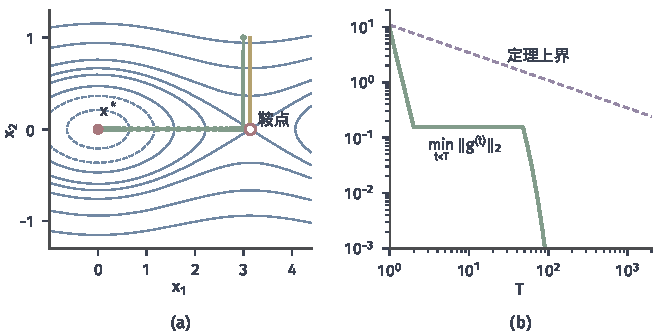
\includegraphics[width=112mm]{figures/05-optimization/02-smooth-optimization/matplotlib/fom-nonconvex/figure.pdf}
  \caption{非凸目标$f(\bm{x})=-\cos x_1+\tfrac92x_2^2$上取$\alpha=1/9$的梯度下降。(a)等高线与两条路径：黄色从$(\pi,1)$出发，终止于鞍点（红色空心点）；绿色从$(3,1)$出发，到达极小点（红点）。(b)绿色路径的$\min_{t<T}\lVert\bm{g}^{(t)}\rVert_2$（绿线），紫色虚线是式~\eqref{eq:fom-gd-nonconvex}的上界开方。中段的平台对应在鞍点附近的徘徊。}
  \label{fig:fom-nonconvex}
\end{BookInlineFigure}

\paragraph{凸情形：目标差}
加上凸性后，局部的谷底就是全局的谷底，可以用目标差来衡量。关键的新工具是：切平面从下方托住目标，用它比较当前点和最优解。

\begin{theorem}[凸情形的梯度下降]
\label{thm:fom-gd-convex}
设$f$凸，梯度$L$-Lipschitz连续，且存在最优解$\bm{x}^\star$。取$\alpha=1/L$，则对任意$T\geq1$，
\begin{equation}
 f(\bm{x}^{(T)})-f^\star\leq\frac{L\lVert\bm{x}^{(0)}-\bm{x}^\star\rVert_2^2}{2T}.
 \label{eq:fom-gd-convex}
\end{equation}
\end{theorem}

\begin{proof}
记$\bm{x}=\bm{x}^{(t)}$，$\bm{x}^+=\bm{x}^{(t+1)}$，$\bm{g}=\bm{g}^{(t)}$。由凸性，切平面在$\bm{x}^\star$处不高于目标：
\[
 f^\star\geq f(\bm{x})+\bm{g}^\top(\bm{x}^\star-\bm{x}).
\]

由式~\eqref{eq:fom-gd-decrease}，$\alpha=1/L$时单步下降至少为$\lVert\bm{g}\rVert_2^2/(2L)$。把上式代入，得到
\[
 f(\bm{x}^+)-f^\star\leq\bm{g}^\top(\bm{x}-\bm{x}^\star)-\frac{1}{2L}\lVert\bm{g}\rVert_2^2.
\]

把$\bm{x}^+=\bm{x}-\bm{g}/L$代入距离的平方，展开得
\[
 \lVert\bm{x}^+-\bm{x}^\star\rVert_2^2
 =\lVert\bm{x}-\bm{x}^\star\rVert_2^2-\frac2L\bm{g}^\top(\bm{x}-\bm{x}^\star)+\frac{1}{L^2}\lVert\bm{g}\rVert_2^2.
\]

两式比较，前一式的右端恰好等于距离平方之差的$L/2$倍：
\[
 f(\bm{x}^{(t+1)})-f^\star\leq\frac L2\Bigl(\lVert\bm{x}^{(t)}-\bm{x}^\star\rVert_2^2-\lVert\bm{x}^{(t+1)}-\bm{x}^\star\rVert_2^2\Bigr).
\]

对$t=0,\ldots,T-1$求和，右端裂项，丢掉末项，得到
\[
 \sum_{t=1}^{T}\bigl(f(\bm{x}^{(t)})-f^\star\bigr)\leq\frac L2\lVert\bm{x}^{(0)}-\bm{x}^\star\rVert_2^2.
\]

函数值逐步下降，所以最后一项是$T$项中最小的，不超过平均值，即得式~\eqref{eq:fom-gd-convex}。
\end{proof}

上面证明还顺带说明，到最优解的距离每步不增。

$1/T$这个阶对梯度下降不能改进。取$f(\bm{x})=\tfrac12(Lx_1^2+\lambda x_2^2)$，$0<\lambda\leq L$，起点的第一坐标为$0$，第二坐标为$x_0$。$\alpha=1/L$时目标差是$\tfrac12\lambda(1-\lambda/L)^{2T}x_0^2$。对每个给定的$T$，取$\lambda=L/(2T)$，因子$(1-1/(2T))^{2T}$接近$\mathrm{e}^{-1}$，于是目标差约为
\[
 \frac{Lx_0^2}{4\mathrm{e}\,T}.
\]
也就是说，曲率总可以小到让梯度下降在这$T$步内几乎察觉不到。这个例子的$\lambda$随$T$变化，它说明上界在整个函数类上的阶不能改进，并不是说某个固定的二次目标只有$1/T$的速度。

\paragraph{强凸情形：线性收敛}
再加上强凸，第~\ref{chap:optimization}章的结论告诉我们解存在且唯一。这时切平面之上还多出一个二次项：
\begin{equation}
 f(\bm{y})\geq f(\bm{x})+\nabla f(\bm{x})^\top(\bm{y}-\bm{x})+\frac\mu2\lVert\bm{y}-\bm{x}\rVert_2^2.
 \label{eq:fom-strong-convexity}
\end{equation}
这是一只从下方托住地面的碗，与式~\eqref{eq:fom-descent-lemma}从上方扣住地面的碗相对。上下两只碗夹住地形，每步的进度就能与当前的误差比较。

\begin{theorem}[强凸情形的梯度下降]
\label{thm:fom-gd-strong}
设$f$的梯度$L$-Lipschitz连续且满足式~\eqref{eq:fom-strong-convexity}，$\mu>0$，$\kappa=L/\mu$。取$\alpha=1/L$，则
\begin{equation}
 \begin{aligned}
 f(\bm{x}^{(T)})-f^\star&\leq\Bigl(1-\frac1\kappa\Bigr)^T\bigl(f(\bm{x}^{(0)})-f^\star\bigr),\\
 \lVert\bm{x}^{(T)}-\bm{x}^\star\rVert_2^2&\leq\Bigl(1-\frac1\kappa\Bigr)^T\lVert\bm{x}^{(0)}-\bm{x}^\star\rVert_2^2.
 \end{aligned}
 \label{eq:fom-gd-strong}
\end{equation}
\end{theorem}

\begin{proof}
先证梯度能控制目标差。在式~\eqref{eq:fom-strong-convexity}中对$\bm{y}$取右端的最小值，最小点是$\bm{y}=\bm{x}-\nabla f(\bm{x})/\mu$，于是
\[
 f^\star\geq f(\bm{x})-\frac{1}{2\mu}\lVert\nabla f(\bm{x})\rVert_2^2,
 \qquad\text{即}\qquad
 \lVert\nabla f(\bm{x})\rVert_2^2\geq2\mu\bigl(f(\bm{x})-f^\star\bigr).
\]

代入式~\eqref{eq:fom-gd-decrease}（$\alpha=1/L$），两边减去$f^\star$，得到
\[
 f(\bm{x}^+)-f^\star\leq\Bigl(1-\frac\mu L\Bigr)\bigl(f(\bm{x})-f^\star\bigr).
\]
迭代$T$次即得第一式。

再证距离。在式~\eqref{eq:fom-strong-convexity}中取$\bm{y}=\bm{x}^\star$，整理得
\[
 \bm{g}^\top(\bm{x}-\bm{x}^\star)\geq f(\bm{x})-f^\star+\frac\mu2\lVert\bm{x}-\bm{x}^\star\rVert_2^2.
\]

另由$f^\star\leq f(\bm{x}^+)$和单步下降，得到
\[
 \lVert\bm{g}\rVert_2^2\leq2L\bigl(f(\bm{x})-f^\star\bigr).
\]

把这两式代入距离平方的展开式：
\[
 \begin{aligned}
 \lVert\bm{x}^+-\bm{x}^\star\rVert_2^2
 &=\lVert\bm{x}-\bm{x}^\star\rVert_2^2-\frac2L\bm{g}^\top(\bm{x}-\bm{x}^\star)+\frac{1}{L^2}\lVert\bm{g}\rVert_2^2\\
 &\leq\Bigl(1-\frac\mu L\Bigr)\lVert\bm{x}-\bm{x}^\star\rVert_2^2-\frac2L\bigl(f(\bm{x})-f^\star\bigr)+\frac2L\bigl(f(\bm{x})-f^\star\bigr).
 \end{aligned}
\]
后两项抵消，迭代$T$次即得第二式。
\end{proof}

用贯穿例核对。$\alpha=1/9$时$\bm{x}^{(1)}=(8,0)$，此后第一坐标每步乘以$8/9$，所以
\[
 f(\bm{x}^{(T)})=32\Bigl(\frac{64}{81}\Bigr)^{T-1},\qquad T\geq1.
\]
定理的上界是$45\cdot(8/9)^T$，$T=1$时是$40$，大于真实值$32$。图~\ref{fig:fom-gd-rates}(a)显示，上界比真实的衰减慢：定理覆盖所有满足条件的函数，这个二次例子并不是最坏的。

\paragraph{条件数怎样影响进展}
三条定理合起来回答了“要多少步”。目标差达到$\varepsilon$所需的步数，凸时约为$LR^2/(2\varepsilon)$，其中$R=\lVert\bm{x}^{(0)}-\bm{x}^\star\rVert_2$；强凸时由$(1-1/\kappa)^T\leq\mathrm{e}^{-T/\kappa}$得到
\[
 T\geq\kappa\ln\frac{f(\bm{x}^{(0)})-f^\star}{\varepsilon}.
\]

所需步数与$\kappa$成正比。把山谷的纵横比拉大十倍，步数也大约变成十倍。图~\ref{fig:fom-gd-rates}(b)对$\operatorname{diag}(1,\kappa)$实测目标差降到初值$10^{-6}$的步数，它紧贴直线$\tfrac\kappa4\ln(1/\varepsilon)$。这里$\tfrac14$来自最佳步长：因子$(\kappa-1)/(\kappa+1)$约为$1-2/\kappa$，目标差的因子是其平方。

\begin{BookInlineFigure}
  \centering
  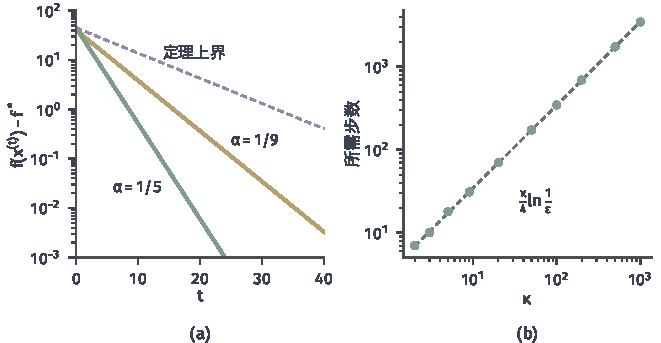
\includegraphics[width=112mm]{figures/05-optimization/02-smooth-optimization/matplotlib/fom-gd-rates/figure.pdf}
  \caption{收敛速度与条件数。(a)贯穿例的目标差：黄线$\alpha=1/9$，绿线$\alpha=1/5$，紫色虚线是$\alpha=1/L$时式~\eqref{eq:fom-gd-strong}的上界$45(8/9)^t$。(b)目标$\tfrac12(x_1^2+\kappa x_2^2)$，起点$(\kappa,1)$，步长$2/(1+\kappa)$，绿点是目标差降到初值$10^{-6}$倍的实测步数，虚线为$\tfrac\kappa4\ln(1/\varepsilon)$，$\varepsilon=10^{-6}$。}
  \label{fig:fom-gd-rates}
\end{BookInlineFigure}

原因已经在式~\eqref{eq:fom-gd-factor}中：步长被陡峭方向限制在$2/L$以内，平坦方向每步只能收缩$\mu/L$量级的比例。下面的表格汇总三种情形。

\begin{BookInlineTable}
  \centering
  \caption{梯度下降$\alpha=1/L$的保证，$\Delta=f(\bm{x}^{(0)})-f_{\inf}$，$R=\lVert\bm{x}^{(0)}-\bm{x}^\star\rVert_2$。}
  \label{tab:fom-gd-summary}
  \begin{tabular}{llll}
   \toprule
   假设 & 度量 & 上界 & 达到$\varepsilon$的步数\\
   \midrule
   非凸，有下界 & $\min_t\lVert\bm{g}^{(t)}\rVert_2^2$ & $2L\Delta/T$ & $2L\Delta/\varepsilon$\\
   凸 & $f(\bm{x}^{(T)})-f^\star$ & $LR^2/(2T)$ & $LR^2/(2\varepsilon)$\\
   强凸 & $f(\bm{x}^{(T)})-f^\star$ & $(1-1/\kappa)^T\Delta$ & $\kappa\ln(\Delta/\varepsilon)$\\
   \bottomrule
  \end{tabular}
\end{BookInlineTable}

表中第一行的$\varepsilon$是梯度平方的容差，所以换成梯度大小达到$\varepsilon$时，步数是$2L\Delta/\varepsilon^2$。三行的度量不同，步数不能直接相比。
